% PUFGuard architecture diagram (Figure 1).
% Standalone: compile with  pdflatex architecture.tex  -> architecture.pdf
\documentclass[border=6pt]{standalone}
\usepackage{tikz}
\usepackage{xcolor}
\usetikzlibrary{positioning,arrows.meta}

\definecolor{pufteal}{HTML}{0F766E}
\definecolor{pufgray}{HTML}{6B7280}
\definecolor{pufhalt}{HTML}{B91C1C}
\definecolor{puflight}{HTML}{E6F2F1}
\definecolor{pufgraybg}{HTML}{EFEFEF}

\begin{document}
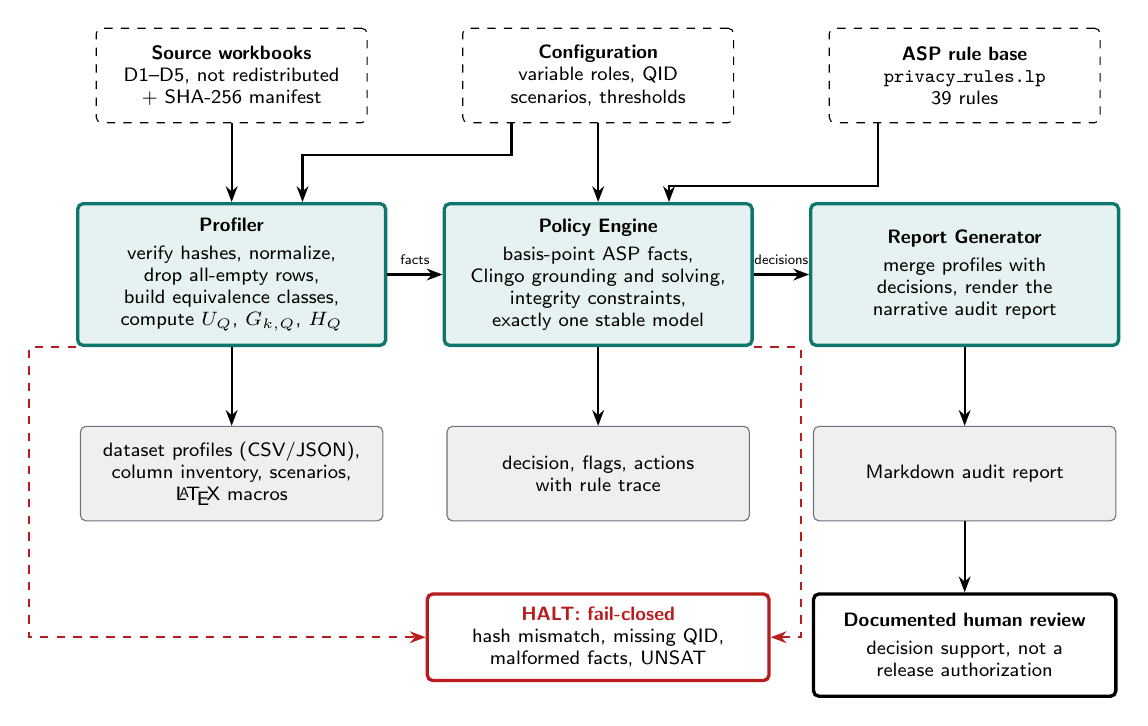
\begin{tikzpicture}[
  font=\sffamily\scriptsize,
  cfgbox/.style = {draw, dashed, rounded corners=2pt, align=center,
                   text width=33mm, minimum height=12mm, inner sep=2pt},
  procbox/.style = {draw=pufteal, very thick, fill=puflight, rounded corners=2pt,
                    align=center, text width=37mm, minimum height=18mm, inner sep=3pt},
  outbox/.style = {draw=pufgray, fill=pufgraybg, rounded corners=2pt, align=center,
                   text width=37mm, minimum height=12mm, inner sep=2pt},
  haltbox/.style = {draw=pufhalt, very thick, rounded corners=2pt, align=center,
                    text width=42mm, minimum height=11mm, inner sep=2pt},
  humanbox/.style = {draw, very thick, rounded corners=2pt, align=center,
                     text width=37mm, minimum height=13mm, inner sep=2pt},
  flow/.style = {-{Stealth[length=2mm]}, thick},
  fail/.style = {-{Stealth[length=2mm]}, thick, dashed, draw=pufhalt},
]

% ---------- configuration inputs (dashed) ----------
\node[cfgbox] (src) {\textbf{Source workbooks}\\ D1--D5, not redistributed\\ + SHA-256 manifest};
\node[cfgbox, right=12mm of src] (cfg) {\textbf{Configuration}\\ variable roles, QID\\ scenarios, thresholds};
\node[cfgbox, right=12mm of cfg] (rules) {\textbf{ASP rule base}\\ \texttt{privacy\_rules.lp}\\ 39 rules};

% ---------- processing components (solid, colored) ----------
\node[procbox, below=10mm of src] (prof) {\textbf{Profiler}\\[2pt] verify hashes, normalize,\\ drop all-empty rows,\\ build equivalence classes,\\ compute $U_Q$, $G_{k,Q}$, $H_Q$};
\node[procbox, below=10mm of cfg] (eng) {\textbf{Policy Engine}\\[2pt] basis-point ASP facts,\\ Clingo grounding and solving,\\ integrity constraints,\\ exactly one stable model};
\node[procbox, below=10mm of rules] (rep) {\textbf{Report Generator}\\[2pt] merge profiles with\\ decisions, render the\\ narrative audit report};

% ---------- generated outputs (gray) ----------
\node[outbox, below=10mm of prof] (o1) {dataset profiles (CSV/JSON),\\ column inventory, scenarios,\\ \LaTeX{} macros};
\node[outbox, below=10mm of eng] (o2) {decision, flags, actions\\ with rule trace};
\node[outbox, below=10mm of rep] (o3) {Markdown audit report};

% ---------- fail-closed ----------
\node[haltbox, below=9mm of o2] (halt) {\textcolor{pufhalt}{\textbf{HALT: fail-closed}}\\ hash mismatch, missing QID,\\ malformed facts, UNSAT};

% ---------- human boundary ----------
\node[humanbox, below=9mm of o3] (human) {\textbf{Documented human review}\\[2pt] decision support, not a\\ release authorization};

% ---------- flows ----------
% source workbooks feed the Profiler; configuration feeds Profiler and Engine;
% the rule base is loaded by the Policy Engine.
\draw[flow] (src) -- (prof);
\draw[flow] (cfg) -- (eng);
\draw[flow] ([xshift=-11mm]cfg.south) -- ++(0,-4mm) -| ([xshift=9mm]prof.north);
\draw[flow] ([xshift=-11mm]rules.south) -- ++(0,-8mm) -| ([xshift=9mm]eng.north);

\draw[flow] (prof) -- node[above, font=\sffamily\tiny] {facts} (eng);
\draw[flow] (eng) -- node[above, font=\sffamily\tiny] {decisions} (rep);

\draw[flow] (prof) -- (o1);
\draw[flow] (eng) -- (o2);
\draw[flow] (rep) -- (o3);

% fail-closed paths leave the processing components, routed clear of the outputs
\draw[fail] (prof.south west) -- ++(-6mm,0) |- (halt.west);
\draw[fail] (eng.south east) -- ++(6mm,0) |- (halt.east);

\draw[flow] (o3) -- (human);

\end{tikzpicture}
\end{document}
